% Results & Discussion — viscode_shared_subspace_probe
% D028 framing: methodological contribution + honest case study
% Generated: 2026-04-11

%% ============================================================
\section{Results}
\label{sec:results}
%% ============================================================

\subsection{Diagnostic Control: Format Identity (F1)}
\label{sec:f1}

A linear format probe (logistic regression, 5-fold CV) achieves \textbf{100\% accuracy at every layer} (L4--L28) for all three models (Table~\ref{tab:probe_accuracy}, Appendix).
This is expected: the three formats occupy near-disjoint vocabulary regions (pairwise token-ID Jaccard $\leq 0.136$; \S\ref{sec:robustness-token}), so a linear classifier can discriminate formats from token identity alone.
A permuted-label baseline (100 permutations) confirms that probe accuracy is at chance (${\approx}\,0.333$) under label shuffling, ruling out $n \ll d$ over-fitting (details in Appendix, Table~\ref{tab:permuted_probe}).
F1 therefore serves as a \textbf{sanity check}: format-specific information dominates hidden representations, and any cross-format signal (F2--F5) is a second-order effect within this format-dominated regime.

\subsection{Cross-Format Representational Similarity (F2)}
\label{sec:f2}

Despite format dominance, we observe statistically significant cross-format representational similarity as measured by linear CKA \cite{kornblith2019similarity}.
Table~\ref{tab:cka_mean} reports the mean CKA across the three unordered format pairs at each layer.

\begin{table}[!ht]
\centering
\small
\caption{Bootstrap mean CKA (linear kernel, 1{,}000 resamples) across format pairs per model at selected layers, with 95\% CI in brackets. Complete per-pair values in Table~\ref{tab:cka_complete} (Appendix).}
\label{tab:cka_mean}
\resizebox{\columnwidth}{!}{%
\begin{tabular}{lccccc}
\toprule
Model & L4 & L12 & L16 & L24 & L28 \\
\midrule
Qwen2.5-Coder & 0.119\,{\scriptsize[.10,.14]} & 0.152\,{\scriptsize[.13,.17]} & 0.174\,{\scriptsize[.15,.20]} & 0.176\,{\scriptsize[.15,.20]} & 0.187\,{\scriptsize[.16,.21]} \\
VisCoder2      & 0.121\,{\scriptsize[.10,.14]} & 0.166\,{\scriptsize[.14,.19]} & 0.179\,{\scriptsize[.16,.20]} & 0.184\,{\scriptsize[.16,.21]} & 0.176\,{\scriptsize[.16,.20]} \\
Qwen2.5 (base) & 0.119\,{\scriptsize[.10,.14]} & 0.144\,{\scriptsize[.13,.16]} & 0.146\,{\scriptsize[.13,.17]} & 0.154\,{\scriptsize[.13,.18]} & 0.099\,{\scriptsize[.08,.12]} \\
\bottomrule
\end{tabular}}
\end{table}

A permutation test (A2; 5{,}000 permutations of format labels) confirms that the observed CKA significantly exceeds chance for all three models ($p < 0.001$; Table~\ref{tab:a2_perm}; Figure~\ref{fig:perm_null}).
The effect is small but statistically reliable: across all three models, observed CKA is $2.76$--$2.96\times$ the permutation null mean (Table~\ref{tab:a2_perm}), a ratio we adopt as effect size throughout.

\begin{table}[!ht]
\centering
\small
\caption{A2 permutation test (5,000 permutations). Observed CKA is the layer-averaged mean across format pairs.}
\label{tab:a2_perm}
\resizebox{\columnwidth}{!}{%
\begin{tabular}{lcccc}
\toprule
Model & Observed & Null mean & Null 95th & $p$-value \\
\midrule
Qwen2.5-Coder  & 0.1226 & 0.0414 & 0.0469 & $<$0.001 \\
VisCoder2       & 0.1243 & 0.0443 & 0.0498 & $<$0.001 \\
Qwen2.5 (base)  & 0.1011 & 0.0366 & 0.0416 & $<$0.001 \\
\bottomrule
\end{tabular}}
\end{table}

\begin{figure}[!ht]
\centering
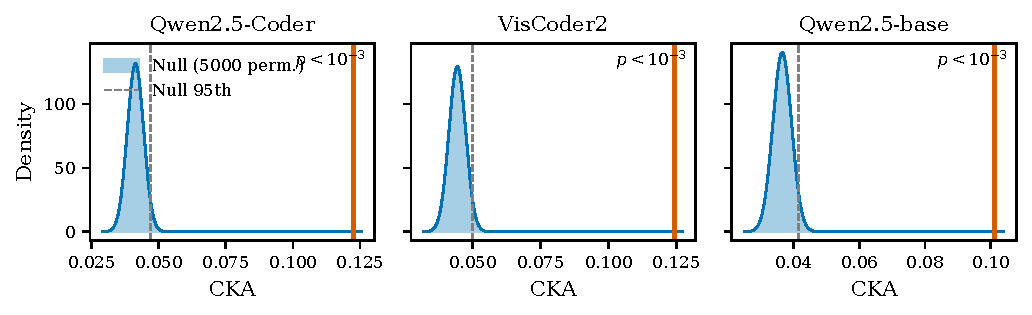
\includegraphics[width=\columnwidth]{fig_permutation_null.pdf}
\caption{A2 permutation null distributions (5,000 permutations) with observed CKA (dashed red). All observed values fall $>$20 standard deviations above the null mean.}
\label{fig:perm_null}
\end{figure}

Bootstrap 95\% confidence intervals (1{,}000 resamples) are narrow across all Qwen model--layer combinations (e.g., Qwen2.5-Coder at L28: $[0.164, 0.212]$; Qwen2.5-Base at L28: $[0.081, 0.122]$), with widths ranging from 0.037 to 0.050, all below the pre-registered threshold of 0.1.
We characterize this as \textbf{statistically significant but weak cross-format representational similarity}: the signal is reliably $2.8$--$3.0\times$ above the permutation null, but bootstrap mean CKA values in the 0.10--0.19 range are small in absolute terms and are dwarfed by the format-specific signal captured by the 100\% probe accuracy.

\begin{figure*}[t]
\centering
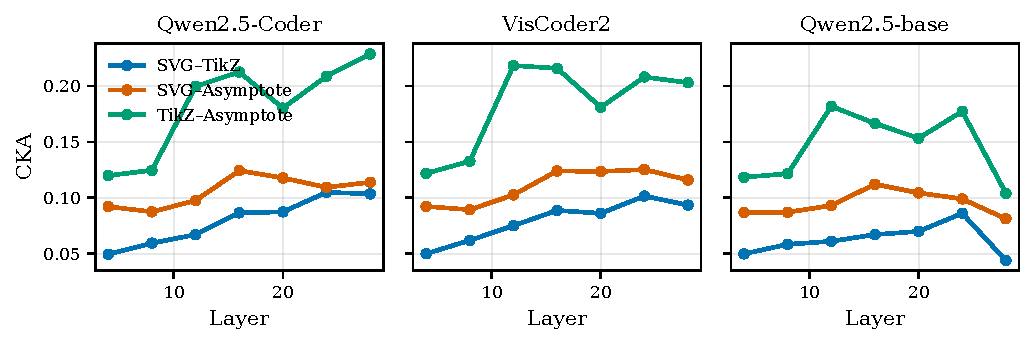
\includegraphics[width=\textwidth]{fig_cka_format_pairs.pdf}
\caption{CKA by format pair across layers. TikZ--Asy consistently exceeds SVG--TikZ by 2--3$\times$ across all models (F3), consistent with a token-overlap gradient modulated by layer-dependent factors (see \S\ref{sec:f3}).}
\label{fig:cka_format_pairs}
\end{figure*}

\subsection{Token-Overlap Gradient (F3)}
\label{sec:f3}

Disaggregating CKA by format pair reveals a systematic asymmetry (Figure~\ref{fig:cka_format_pairs}, Table~\ref{tab:cka_pairs}).
Across all models and layers, the TikZ--Asy pair yields CKA values 2--3$\times$ higher than the SVG--TikZ pair.
At L28 for Qwen2.5-Coder, TikZ--Asy CKA is 0.229 versus SVG--TikZ at 0.103 ($2.2\times$); at L12 for Qwen2.5 base, the ratio is $0.182 / 0.061 = 3.0\times$.

\begin{table}[!ht]
\centering
\small
\caption{CKA by format pair at selected layers (Qwen2.5-Coder shown; other models follow the same pattern).}
\label{tab:cka_pairs}
\begin{tabular}{lccc}
\toprule
Layer & SVG--TikZ & SVG--Asy & TikZ--Asy \\
\midrule
L4  & 0.049 & 0.092 & 0.120 \\
L12 & 0.067 & 0.098 & 0.200 \\
L16 & 0.086 & 0.124 & 0.212 \\
L24 & 0.105 & 0.109 & 0.209 \\
L28 & 0.103 & 0.114 & 0.229 \\
\bottomrule
\end{tabular}
\end{table}

The pair-level CKA ordering follows BPE token Jaccard similarity (Spearman $\rho \approx 0.7$ over 6 pairs), establishing lexical overlap as a necessary driver of the observed asymmetry.
Using the Qwen2.5-Coder tokenizer on the 252 prompts, token-type Jaccard is highest for TikZ--Asy (0.111), followed by SVG--Asy (0.091) and SVG--TikZ (0.087); Python--visual pairs are substantially lower (0.021--0.039).
However, the cell-level rank correlation attenuates to $\rho = 0.57$ across 126 cells (6 pairs $\times$ 3 models $\times$ 7 layers, $p < 10^{-11}$), and the CKA-to-Jaccard magnitude ratio varies from 0.9 (SVG--TikZ) to 2.9 (Python--SVG), growing at mid/late layers where Jaccard is constant.
We therefore attribute F3 to a \textbf{token-overlap gradient modulated by layer-dependent representational factors}: lexical similarity provides the ordering but cannot alone explain the layer-specific amplification in deeper layers (\S\ref{sec:disc-syntax}).

The C1 Python control (\S\ref{sec:c1}) provides additional evidence: python-pair asymmetry mirrors visual-pair asymmetry at similar lexical distances (python--tikz Jaccard 0.039 vs.\ python--svg 0.021, ratio 1.9$\times$; corresponding CKA ratio 1.5--2.3$\times$ across 20/21 cells).

\begin{figure*}[t]
\centering
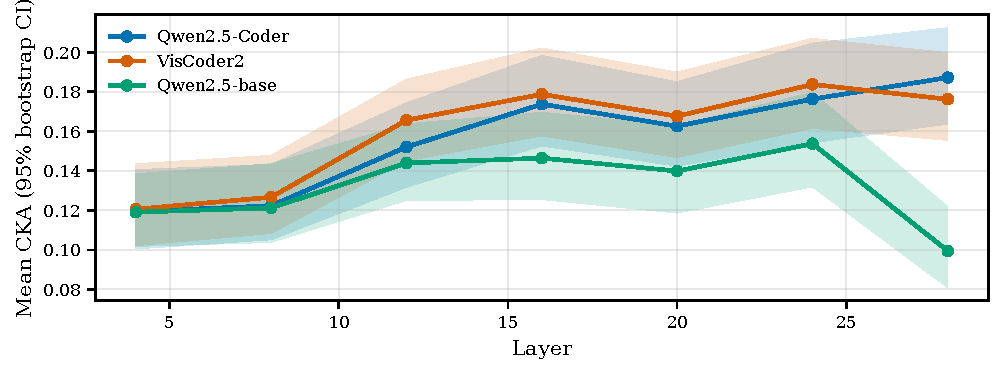
\includegraphics[width=\textwidth]{fig_cka_trajectories.pdf}
\caption{Layer-wise mean CKA trajectories with 95\% bootstrap confidence intervals. Qwen2.5-Base exhibits a sharp drop at L28 (F4), while instruction-tuned models plateau or continue increasing.}
\label{fig:cka_layer}
\end{figure*}

\subsection{Layer-wise Dynamics (F4)}
\label{sec:f4}

Within the Qwen family, the three models exhibit qualitatively different layer-wise CKA trajectories (Figure~\ref{fig:cka_layer}).
Qwen2.5-Coder shows a broadly rising profile (bootstrap mean 0.119 at L4 to 0.187 at L28), while VisCoder2 plateaus in the upper layers (peak 0.184 at L24).
Qwen2.5 base follows a similar rising trend from L4 (0.119) to L24 (0.154), but undergoes a \textbf{sharp drop at L28} (0.099), a 36\% decrease from L24.

This divergence at the final probed layer is consistent across all three format pairs for Qwen2.5 base (SVG--TikZ: $0.086 \to 0.044$; SVG--Asy: $0.099 \to 0.081$; TikZ--Asy: $0.177 \to 0.104$) and is corroborated by Procrustes distance (L24: 0.137 $\to$ L28: 0.094; \S\ref{sec:robustness-procrustes}).
The C1 negative control data (\S\ref{sec:c1}) reveals that this washout is amplified for non-visual code: over the L24$\to$L28 interval, Qwen2.5~base python-X CKA drops from 0.075 to 0.030 ($-60\%$), compared with visual-X CKA from 0.121 to 0.076 ($-37\%$, cross-validating the F2 data of $0.154 \to 0.099 = -36\%$).
Over the same L24$\to$L28 interval, Coder (python $+11\%$, visual $+5\%$) and VisCoder2 (python $+4\%$, visual $-5\%$) show no comparable washout on either signal; the VisCoder2 visual $-5\%$ is within the bootstrap fluctuation envelope and does not replicate Qwen2.5-base's $-37\%$ drop.
The larger magnitude of the python drop reflects that the already-weak python-X signal is driven below the permutation null at L28, whereas the visual signal, though diminished, remains above chance.
We therefore interpret F4 as Qwen2.5-base's final-layer destabilization of residual cross-format alignment, rather than as evidence that non-visual code had meaningful mid-layer structure to lose.
The washout is therefore a Qwen2.5-base-specific phenomenon at the final probed layer, not a general property across models or modalities.

\subsection{Effect of Visual-Code SFT (F5)}
\label{sec:f5}

VisCoder2 is fine-tuned from Qwen2.5-Coder on VisCode-Multi-679K, a 679K-example multi-format visual code SFT corpus \cite{viscoder2}.
Despite this additional training, the two models exhibit nearly identical CKA profiles: at L28, Qwen2.5-Coder reaches a bootstrap mean of 0.187 $[0.164, 0.212]$ and VisCoder2 reaches 0.176 $[0.155, 0.200]$, with broadly overlapping confidence intervals.
The maximum bootstrap mean difference between the two models is 0.011 (at L28).

This suggests that SFT on visual code data does not substantially alter the underlying cross-format representational structure.
However, this comparison carries a \textbf{contamination caveat}: VisCoder2's SFT training data (VCM-Asy) overlaps with the probe pool source for Asymptote, establishing a memorization floor that may inflate its CKA values for Asy-related pairs.
The near-equivalence between the two models should therefore be interpreted cautiously.

\subsection{Cross-Architecture Generalizability}
\label{sec:generalizability}

To test whether the cross-format signal generalizes beyond the Qwen family, we extend the analysis to three architecturally diverse models: Codestral-22B (Mistral, 56 layers), StarCoder2-15B (BigCode, 40 layers), and DeepSeek-Coder-V2-Lite (MoE, 27 layers).
For each model, we extract hidden states at 7 equidistant layers via the formula $\lfloor n_\text{layers} \cdot (i+1)/7 \rceil$ and repeat the full CKA analysis pipeline (252 triples, 5{,}000 A2 permutations, 1{,}000 bootstrap resamples).
Table~\ref{tab:cross_arch} reports bootstrap mean peak CKA with 95\% CI and obs/null ratios.

\begin{table}[!ht]
\centering
\small
\caption{Cross-architecture CKA summary (6 models, 4 architecture families). Peak CKA is the bootstrap mean at the highest-CKA layer. Obs/null ratio is the A2 permutation effect size.}
\label{tab:cross_arch}
\resizebox{\columnwidth}{!}{%
\begin{tabular}{llcccl}
\toprule
Model & Arch & Peak [95\% CI] & Depth & Ratio & Profile \\
\midrule
Codestral-22B & Mistral & 0.190\,[0.178, 0.203] & 57\% & 3.01$\times$ & inverted-U \\
Qwen2.5-Coder-7B & Qwen & 0.187\,[0.164, 0.212] & 100\% & 2.96$\times$ & broadly rising \\
VisCoder2-7B & Qwen & 0.184\,[0.162, 0.207] & 86\% & 2.81$\times$ & late-plateau \\
StarCoder2-15B & BigCode & 0.164\,[0.152, 0.177] & 100\% & 2.55$\times$ & bimodal \\
DeepSeek-V2-Lite & MoE & 0.155\,[0.145, 0.167] & 56\% & 2.75$\times$ & inverted-U \\
Qwen2.5-7B & Qwen & 0.154\,[0.132, 0.180] & 86\% & 2.76$\times$ & late-plateau \\
\bottomrule
\end{tabular}}
\end{table}

All six models yield $p < 0.001$ with obs/null ratios in the narrow band of $2.55$--$3.01\times$, confirming that the weak cross-format signal is not Qwen-specific.
The TikZ--Asy $>$ SVG--Asy $>$ SVG--TikZ ordering holds universally, strengthening the token-overlap gradient (F3) as a cross-architecture finding.

\paragraph{Architecture-dependent layer profiles.}
CKA is lowest in shallow layers ($<$30\% depth) across all models, but peak location varies markedly:
\emph{inverted-U} profiles (Codestral, DeepSeek) peak at ${\sim}$57\% depth with subsequent decline;
\emph{broadly rising} (Qwen2.5-Coder) increases through the final layer with a minor dip at L20;
\emph{late-plateau} models (VisCoder2, Qwen2.5) reach a broad plateau at 60--85\% depth;
and StarCoder2 exhibits a \emph{bimodal W-shape} with an early spike at L11 (28\% depth, bootstrap mean 0.162) and a late peak at L40 (100\%, 0.164), the two peaks having fully overlapping 95\% CIs.
The StarCoder2 L11 spike is driven by an unusually high tikz-asy CKA of 0.259---the single highest pair-layer value across all six models.
These results rule out any universal ``mid-layer peak'' characterization: peak depth is architecture-dependent, ranging from 56\% to 100\%.

\begin{figure}[!ht]
\centering
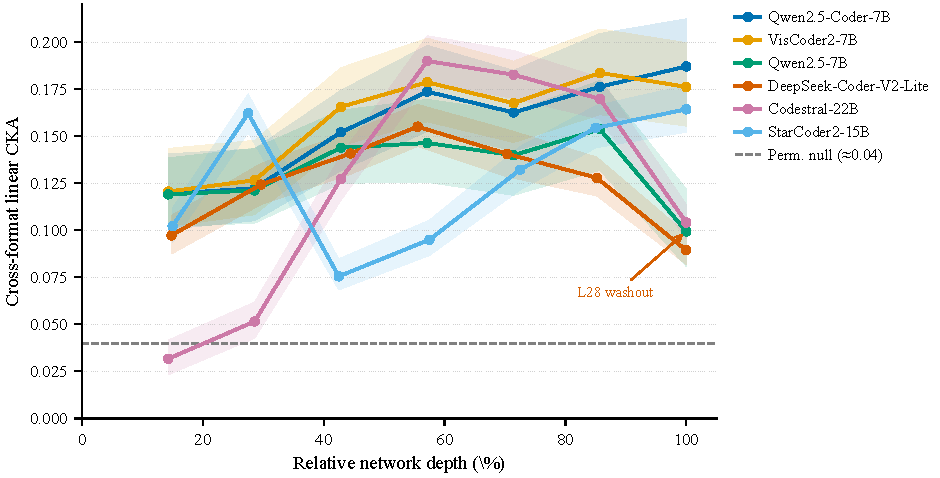
\includegraphics[width=\columnwidth]{figures/fig_cka_layer_curves_6model.pdf}
\caption{Bootstrap mean CKA (with 95\% CI shading) as a function of relative layer depth for six models across four architecture families. Colors encode profile type: inverted-U (Codestral, DeepSeek), bimodal (StarCoder2), broadly rising (Qwen2.5-Coder), and late-plateau (VisCoder2, Qwen2.5). The dashed grey line indicates the approximate permutation null (${\sim}0.04$).}
\label{fig:cka_layer_curves}
\end{figure}

\subsection{Negative Control: Non-Visual Code (C1)}
\label{sec:c1}

To test whether the cross-format signal is visual-specific, we conduct a pre-registered negative control (criterion D060, frozen before data collection).
We teacher-force 252 randomly sampled Python snippets through the three Qwen models and compute CKA between each Python--visual format pair (python--svg, python--tikz, python--asy) at all 7 layers (L4--L28), with 5{,}000 permutations for significance testing.
The design yields 3~models $\times$ 7~layers $\times$ 3~pairs = 63 python-X cells, directly comparable to the 63 visual-X cells (svg--tikz, svg--asy, tikz--asy) from the same experiment.

\paragraph{Magnitude (M1).}
The pre-registered criterion requires mean python-X CKA $< 0.5 \times$ mean visual-X CKA at each (model, layer) pair.
This criterion fails at 20 of 21 cells: python-X CKA ranges from 60--110\% of visual-X CKA across models and layers (Appendix Table~\ref{tab:c1_python_magnitude}).
The sole passing cell is Qwen2.5~base at L28 (python mean 0.030 vs.\ visual mean 0.076), driven by the sharp final-layer washout (F4) that depresses \emph{both} signals.
A second criterion (M2) further requires that permutation testing distinguish python from visual pairs (python $p > 0.05$ with visual $p < 0.001$), and a joint criterion (M3) requires $\geq 3$ models to satisfy both M1 and M2 at the same layer.

\paragraph{Early-layer homogeneity.}
At L4 and L8, all three models show python-X CKA within 80--120\% of visual-X CKA (anti-spin triggered), with python occasionally \emph{exceeding} visual (e.g., coder L4: ratio 1.06, qwen25 L4: 1.11).
Visual-X pairs at these layers also show weaker significance (L4: svg--tikz $p = 0.003$, failing the $p < 0.001$ threshold).
This early-layer convergence is consistent with the well-documented finding that lower transformer layers encode generic token-level features before task-specific structure emerges in deeper layers \cite{jawahar2019bert, tenney2019bert}.

\paragraph{Overall C1 verdict: FAIL.}
Per the pre-registered D060 criterion, C1 is declared FAIL: three independent fail modes are triggered (M1 magnitude at 20/21 cells; M3 joint criterion at 0/7 layers; anti-spin window at 6 cells in L4/L8).
The C1 result establishes that the measured cross-format CKA reflects code-general structure rather than visual-specific representations.

\paragraph{Scope: code-pretrained models only.}
An exploratory ablation with code-naive Llama-3-8B across 7 equidistant layers (Appendix~\ref{sec:llama-baseline}; D075, post-hoc) reveals that while visual cross-format CKA persists at comparable magnitude (21/21 cells $p < 0.005$), the python--visual entanglement does not arise (20/21 cells $p > 0.05$; the sole exception is python--Asy at L8 with borderline $p = 0.039$).
This indicates that the C1 failure mode---where python code yields 60--110\% of visual CKA---is specific to code-pretrained LLMs, not a general property of language models.

\subsection{Robustness Checks}
\label{sec:robustness}

\subsubsection{Procrustes Distance}
\label{sec:robustness-procrustes}

Orthogonal Procrustes distance (with PCA projection to $k=50$ dimensions) shows trends consistent with CKA across all models and layers.
Mean Procrustes values range from 0.094 to 0.158 (Table~\ref{tab:procrustes_mean}), with Qwen2.5 base at L28 again the lowest (0.094), confirming the layer-wise dynamics observed with CKA.

\begin{table}[!ht]
\centering
\small
\caption{Mean Procrustes distance (PCA $k$=50) per model at selected layers.}
\label{tab:procrustes_mean}
\resizebox{\columnwidth}{!}{%
\begin{tabular}{lccccc}
\toprule
Model & L4 & L12 & L16 & L24 & L28 \\
\midrule
Qwen2.5-Coder  & 0.102 & 0.138 & 0.158 & 0.157 & 0.153 \\
VisCoder2       & 0.102 & 0.142 & 0.157 & 0.158 & 0.146 \\
Qwen2.5 (base)  & 0.100 & 0.127 & 0.133 & 0.137 & 0.094 \\
\bottomrule
\end{tabular}}
\end{table}

\subsubsection{PWCCA (Auxiliary)}
\label{sec:robustness-pwcca}

PWCCA \cite{morcos2018pwcca} values (0.78--0.81 across all models) are directionally consistent with the CKA findings.
However, discriminative power is limited in the $n \ll d$ regime ($n{=}252$, $d$ up to $6{,}144$), where baseline canonical correlations are inflated, and we do not make significance claims based on PWCCA alone.
Procrustes distance, which does not suffer from this inflation, is a more reliable robustness check and shows trends fully consistent with CKA (\S\ref{sec:robustness-procrustes}).

\subsubsection{Token-Level Control}
\label{sec:robustness-token}

As an independent control analysis (computed over the full training corpora, not the probe pool), all three models share an identical Qwen2.5 tokenizer (151{,}643 vocabulary entries).
Pairwise token-ID Jaccard similarity between format corpora is uniformly low: SVG--TikZ = 0.025, SVG--Asy = 0.035, TikZ--Asy = 0.136.
The three-way token intersection covers only 1.2\% of the token union.
Format-exclusive tokens constitute $>$46\% of each format's active vocabulary.
This confirms that the 100\% format probe accuracy (\S\ref{sec:f1}) is a tokenization artifact: near-orthogonal token distributions allow perfect classification without relying on learned representations.

\subsubsection{Statistical Power}
\label{sec:robustness-power}

A1 power simulation (1{,}000 Monte Carlo iterations at layer L24) yields power = 1.0 for both $N{=}12$ (headline) and $N{=}18$ (auxiliary) configurations.
The observed CKA across all models (layer-averaged means: 0.123 for Coder, 0.124 for VisCoder2, 0.101 for base; Table~\ref{tab:a2_perm}) far exceeds the permutation null 95th percentile in every case.
This confirms that the permutation test has adequate power to detect CKA signals of the observed magnitude; it does not, however, confirm that the effect size is practically meaningful.


%% ============================================================
\FloatBarrier
\section{Discussion}
\label{sec:discussion}
%% ============================================================

The CKA signal ($2.55$--$3.01\times$ the permutation null across six models) is a second-order effect within representations overwhelmingly organized by format.
We cannot determine from CKA alone whether this reflects (a)~shared visual semantics, (b)~shared syntactic patterns, or (c)~artifacts of shared concept/prompt structure, and characterize it as \textbf{cross-format representational similarity of uncertain origin}.
The TikZ--Asy $\gg$ SVG--TikZ asymmetry (\S\ref{sec:f3}), which holds across all six models and four architecture families, tracks BPE token Jaccard at pair level ($\rho \approx 0.7$), establishing lexical overlap as a primary driver \cite{jawahar2019bert, hewitt-manning-2019-structural}.
The cell-level attenuation ($\rho = 0.57$) and layer-dependent CKA-to-Jaccard ratio growth indicate that tokenization alone does not fully account for the signal.
\label{sec:disc-syntax}
The pre-registered C1 negative control (\S\ref{sec:c1}) further constrains interpretation: python-X CKA reaches 60--110\% of visual-X CKA in magnitude, formally failing the D060 criterion at 20/21 (model, layer) cells.
This establishes that code-general structure---rather than visual-specific representations---dominates the measured alignment.

\paragraph{Split hypothesis (exploratory, D075).}
An ablation with code-naive Llama-3-8B across 7 equidistant layers (Appendix~\ref{sec:llama-baseline}) suggests a two-track interpretation:
(1)~visual cross-format CKA persists at comparable magnitude without code pretraining (21/21 cells $p < 0.005$), indicating that visual code formats share representational structure in general-purpose LLMs;
(2)~python--visual entanglement is substantially stronger in code-pretrained models: Qwen family python-X CKA reaches 60--110\% of visual-X magnitude (D060), whereas Llama-3-8B python-X cells are overwhelmingly non-significant (20/21 cells $p > 0.05$; sole exception: python--Asy L8, $p = 0.039$), suggesting that the C1 failure mode is a code-pretraining artifact.
We note that the 7-layer equidistant protocol samples to L28 (87.5\% depth), missing the final layers where the original three-layer scan (D075) found its only two significant python cells (L31, 97\% depth); python--visual entanglement in code-naive models, if present, may thus be confined to the deepest layers.
This observation is post-hoc and exploratory; confirmation requires pre-registered replication across additional code-naive architectures.

\paragraph{Methodological caveats.}
The fixed sample size ($n{=}252$ triples) constrains all models to the same statistical power, which may compress inter-model differences in CKA magnitude.
Additionally, the obs/null ratio ($2.55$--$3.01\times$) is more comparable across models than absolute CKA values, which vary with hidden dimensionality and model scale.

Key directions for resolving the origin ambiguity include: (1)~format-residualized CKA to project out the format-specific subspace; (2)~caption-conditioned partial correlation to isolate visual-specific signal; and (3)~visually-paired datasets where identical scenes are rendered in all three formats.
